%
%                  Politecnico di Milano
%
%         Student: Caravano Andrea, Alberto Cantele
%            A.Y.: 2024/2025
%
%   Last modified: 25/05/2025
%
%     Description: Internet of Things: Homework
%                  Exercise n. 1
%

\documentclass[a4paper,11pt]{article} % tipo di documento
\usepackage[T1]{fontenc} % codifica dei font
\usepackage[utf8]{inputenc} % lettere accentate da tastiera
\usepackage[english]{babel} % lingua del documento
\usepackage{lipsum} % genera testo fittizio
\usepackage{url} % per scrivere gli indirizzi Internet e/o di riferimento nella pagina

\usepackage{hyperref} % per modificare il comportamento dei collegamenti ipertestuali

\usepackage[margin=0.7in]{geometry} % margine di pagina

\usepackage{graphicx} % per inserire immagini

\usepackage{minted} % per colorazione automatica del codice (installare pygments da Homebrew)
% \usepackage{pythonhighlight} % per Python

\setminted{ % si può impostare il linguaggio specifico con \setminted[JSON] ad esempio
    linenos=true,
    breaklines=true,
    encoding=utf8,
    fontsize=\normalsize,
    frame=lines
}

\usepackage{fancyhdr}
\usepackage{textcomp}
\usepackage{siunitx} % per gestione intestazione e piè di pagina

\usepackage{tcolorbox} % per riquadrature di vario colore

\usepackage{float} % per figure comparative flottanti
\usepackage{amsmath} % per frazioni in display style

\usepackage{icomma} % virgola come separatore decimale

\usepackage{titlesec} % per configurazione del tipo paragrafo

\usepackage{multirow} % righe multiple in tabelle

\usepackage{subfig} % descrizione sottostante a figure

% setup del tipo paragrafo
\setcounter{secnumdepth}{4}

\titleformat{\paragraph}
{\normalfont\normalsize\bfseries}{\theparagraph}{1em}{}
\titlespacing*{\paragraph}
{0pt}{3.25ex plus 1ex minus .2ex}{1.5ex plus .2ex}

\hypersetup{ % metadati di titolo e autore nel PDF
    hidelinks, % leva colore attorno collegamenti ipertestuali
    pdftitle={Internet of Things: Homework - exercise n. 1},
    pdfauthor={Andrea Caravano, Alberto Cantele}
}

\setlength{\parindent}{0pt} % rimuove l'indentazione del testo

\tcbset{ % impostazioni per riquadrature
    colback=gray!20,
    colframe=black,
    boxrule=0.5pt
}

\captionsetup{labelformat=empty} % rimuove la caption delle figure

% Imposta la profondità dell'indice a 2 livelli (sottosezioni, non sotto-sottosezioni)
\setcounter{tocdepth}{2}

\pagestyle{fancy}
\fancyhead{}\fancyfoot{}
\fancyhead[L]{\textbf{Internet of Things: Homework - exercise n. 1}}
\fancyhead[R]{Andrea Caravano, Alberto Cantele}
\fancyfoot[C]{\thepage}

\title{\textbf{Internet of Things}\\Homework: exercise n. 1}
\author{Andrea Caravano, Alberto Cantele}
\date{Academic Year 2024--25}

\begin{document}
\maketitle

%\tableofcontents

\section*{Exercise text}
\subsection*{Context}
A logistics company operates a warehouse composed of a 500 $m^2$ \textbf{underground} indoor area and a 1 $km^2$ outdoor yard.

Electric forklifts are used across both zones and return to specific docking stations to recharge.
\subsection*{Objective}
Design a low-cost IoT system to:
\begin{enumerate}
    \item localize forklifts in real time
    \item monitor their status, including daily distance traveled, maximum and average speed, and impact detection.
\end{enumerate}
\subsection*{Requirements}
Your design must include:
\begin{itemize}
    \item A description of the hardware installed on each forklift, including sensors, processing unit, and communication module.
    \item The chosen connectivity strategy, communication protocol, and data transmission frequency.
    \item A backend architecture detailing how data is ingested, processed, stored, and visualized.
    \item Pseudocode outlining the core logic running on each forklift (data collection, impact detection, communication)
    \item \textbf{A graphical system-wide building block diagram} showing the architecture from edge devices to the backend platform, including key data flows and system components.
\end{itemize}
\textbf{Solutions should prioritize simplicity, low cost, and scalability.}

\textbf{Design choices must be clearly justified.}

\section{Forklift hardware planning}
\hyperref[communication]{As will be discussed later}, the chosen communication technology may be a dictating factor for some hardware component:
in our \textsc{IoT} implementation, however, most hardware devices will be independent of the communication details: we will complete the remaining elements upon planning of the \hyperref[data-exchange]{data-exchange strategy}.

\newpage

In the following, a sketched hardware plan is outlined:

\medskip

\begin{tabular}{|l|l|}
    \hline
    \textbf{Objective}        & \textbf{Hardware device}        \\
    \hline
    Custom monitoring and localization routines & Micro-controller and related circuitry \\
    \hline
    Localization + communication & Wireless connectivity module \\
    \hline
    Monitoring & Inertial Measurement Unit (IMU) \\
    \hline
    Impact detection & Ultrasonic distance sensor \\
    \hline
    Outdoor tracking support & Global Positioning System (GPS) sensor \\
    \hline
    Regular maintenance & Docking station adapter and integrated storage \\
    \hline
\end{tabular}

\medskip

Let's now be more precise in the description of the proposed usage for each component:

\begin{itemize}
    \item Micro-controller board and related circuitry (e.g. ESP-32/Arduino): the processing unit and communication manager of the overall system.

        It will implement the complete monitoring and localization strategies \hyperref[localization]{sketched later}.
    \item Wireless connectivity module (e.g. LoRaWAN/Wi-Fi): wireless communication parameters (e.g. RSSI) can also be used for localization through the \textsc{Fingerprinting} or \textsc{Triangulation} technique, \hyperref[localization]{detailed further on}.
    \item Intertial Measurement Unit (IMU): an IMU is defined as a 9 axis sensor that measures orientation, velocity and gravitational forces by combining an accelerometer, a gyroscope and a magnetometer.

        Its recent iterations are smaller than ever and therefore particularly well suited for micro-controllers and development boards.

        In its essence, an IMU can be used to determine the forklift's orientation and speed for monitoring.

        Note, however, that it may not be a particularly precise solution in the long run: a re-calibration and/or filtering strategy provide optimal results, especially if combined with the docking/recharging procedures.
    \item Ultrasonic distance sensor (e.g. HC-SR04): an ultrasonic distance sensor is an affordable distance measurement sensor, with a range from $\sim 2\ cm$ to $\sim 4\ m$. Its proposed purpose is the implementation of the impact detection routine.

        A measurement cycle is proportional to the duration of the \textsc{ECHO} pulse through a conversion factor.
    \item Global Positioning System (GPS) sensor: the \textsc{Global Positioning System} is the well-known tracking and navigation structure, exhibiting a medium localization precision. It requires, of course, satellite coverage, which excludes the \textsc{underground} area.

        Its current implementation may not be precise enough to track forklifts in the environment: it can serve as a rough support for outdoor tracking, being also sensibly cheap.
    \item Docking station adapter and integrated storage: the docking station serves the purpose of providing energy to the overall system, as expected.

        The integrated storage may be flushed at recharge times to perform a monitoring comparison and complete eventually unavailable data due to communicative inabilities (collisions, congestion, \dots).
\end{itemize}

\section{Localization in wireless networks}\label{localization}
Almost all location systems are composed of two parts:

\smallskip

\begin{itemize}
    \item Anchor nodes: devices in known positions (e.g. GPS satellites)
    \item Target nodes: devices to be localized (e.g. forklifts)
\end{itemize}

\smallskip

Anchor nodes may transmit or receive from the target nodes, depending on the application perspective.

\medskip

Localization systems may be further classified based on:

\begin{itemize}
    \item Signal type: in our case, the most interesting setting are radio-frequency signals.
    \item Type of input data: in our case, the most interesting setting are power-based parameters (e.g. \textsc{Received Signal Strength}, RSS).
    \item Localization technique:
        \begin{enumerate}
            \item Parametric: model-based
            \item Non-parametric: fingerprinting
        \end{enumerate}
\end{itemize}

\subsection{Model-based RSS localization}

\subsubsection{Ranging}

At the receiver, estimate the distance $d$ of the transmitter given the signal strength $s$.

\smallskip

Typically, the \textsc{log-distance path loss model} is used:

\medskip

$s = s_0 - 10 \cdot a \cdot log_{10} \dfrac{d}{d_0} + b$

\medskip

In which:

\begin{itemize}
    \item $s_0$ is the power emitted at $d_0$ meters
    \item $a$ is the path loss exponent, $b$ is a noise term
    \item $s_0$, $a$ are estimated, $b$ is generally set to 0
\end{itemize}

\smallskip

And to finally retrieve $d$:

\medskip

$d = 10^{\dfrac{s_0-s}{10 \cdot a}}$

\subsubsection{Triangulation}\label{triangulation}

The target estimates distances $d_1, d_2, \dots, d_n$ from $n$ anchor nodes in positions $\left(x_1, y_1\right), \left(x_2, y_2\right), \dots, \left(x_n, y_n\right)$.

\smallskip

\begin{center}
    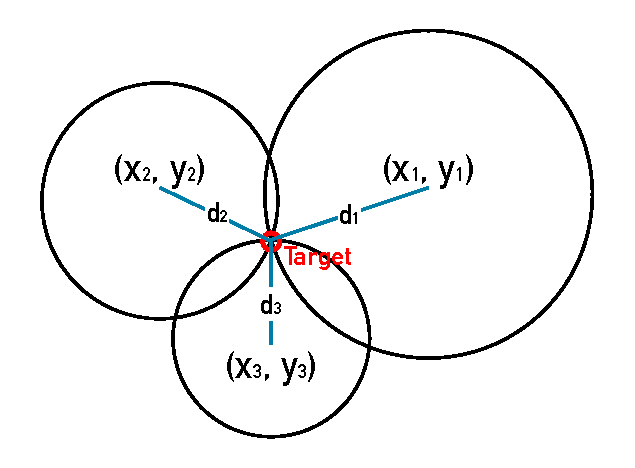
\includegraphics[width=8cm]{../res/triangulation-theory}
\end{center}

\smallskip

Target position is the intersection of the (at least three, of course) circumferences having $d_1, d_2, \dots, d_n$ as radius and $\left(x_1, y_1\right), \left(x_2, y_2\right), \dots, \left(x_n, y_n\right)$ as their centers.

\subsection{Fingerprint-based localization}

The \textsc{fingerprinting} approach consists of two basic steps:

\begin{enumerate}
    \item Construct a radio map (\textsc{fingerprint database}) of the environment, storing for each position $\left(x, y\right)$ the RSS from all visible monitoring points $\left(s_1, s_2, \dots, s_n\right)$.
    \item When the target needs to be localized, transmit the \textsc{RSS} from monitoring points to the database and get the position with the most similar fingerprint.
\end{enumerate}

\medskip

A sketched example of a \textsc{fingerprinting database} construction on a sample underground field is shown in the following

\begin{center}
    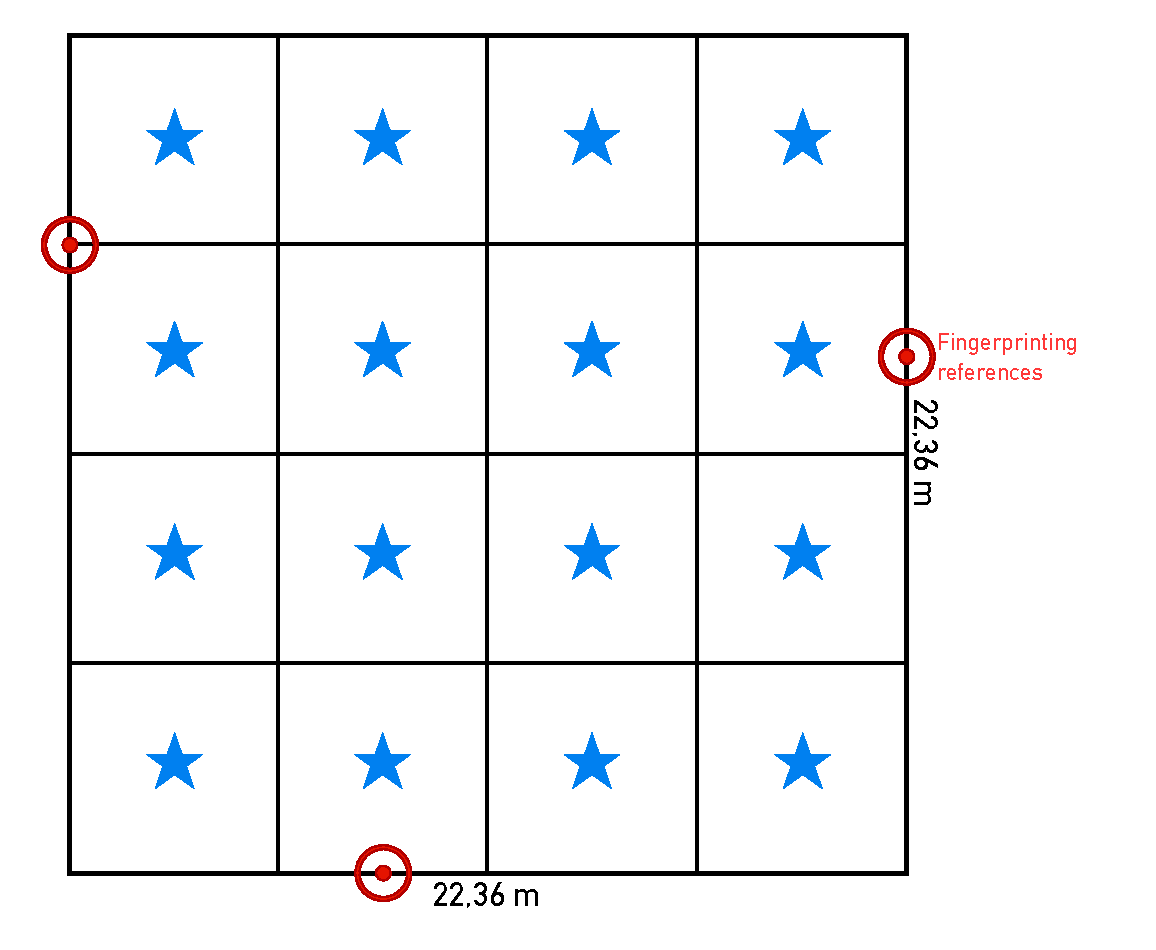
\includegraphics[width=12.5cm]{../res/fingerprint-db-construction}
\end{center}

\section{Communication and connectivity strategy}\label{communication}
\subsection{Communication technologies: a brief overview}
The most relevant communication technology for our case should definitely stem from the considerations about the fields' size and overall running environment.

\smallskip

A \textsc{Wi-Fi} or \textsc{Bluetooth} network seems difficult to fit in such an implementation scenario: being both areas quite large and mobile devices pervasive in the environment, our attention may be focused towards solutions employing \textsc{Long Range} technologies, that also empathize on system's lifetime.

\smallskip

Moreover, as known, \textbf{\textsc{Wi-Fi} or \textsc{Bluetooth} traffic heavily suffers from interference with standard human usage and collisions}, especially at its lowest frequency band (2,4 GHz), being heavily employed in human activities.

\smallskip

Short range technologies instead, like \textsc{ZigBee}, could be adequate only if planning correctly the environment and its distribution, because of the limited transmissive power.

\smallskip

\label{challenge-lorasim}

As inspected during the latest \textsc{Challenge} activity, \textbf{\textsc{LoRaWAN} deployments can hugely benefit from optimizations} on airtime through configuration of transmit parameters, as shown by the following experimental run through \textsc{LoRaSim}, that exhibits a \textsc{Data Extraction Rate (DER)} $\geq 0,9$ in highly polluted transmission environments, while also covering considerable distances ($\sim$ hundreds meters).

\begin{center}
    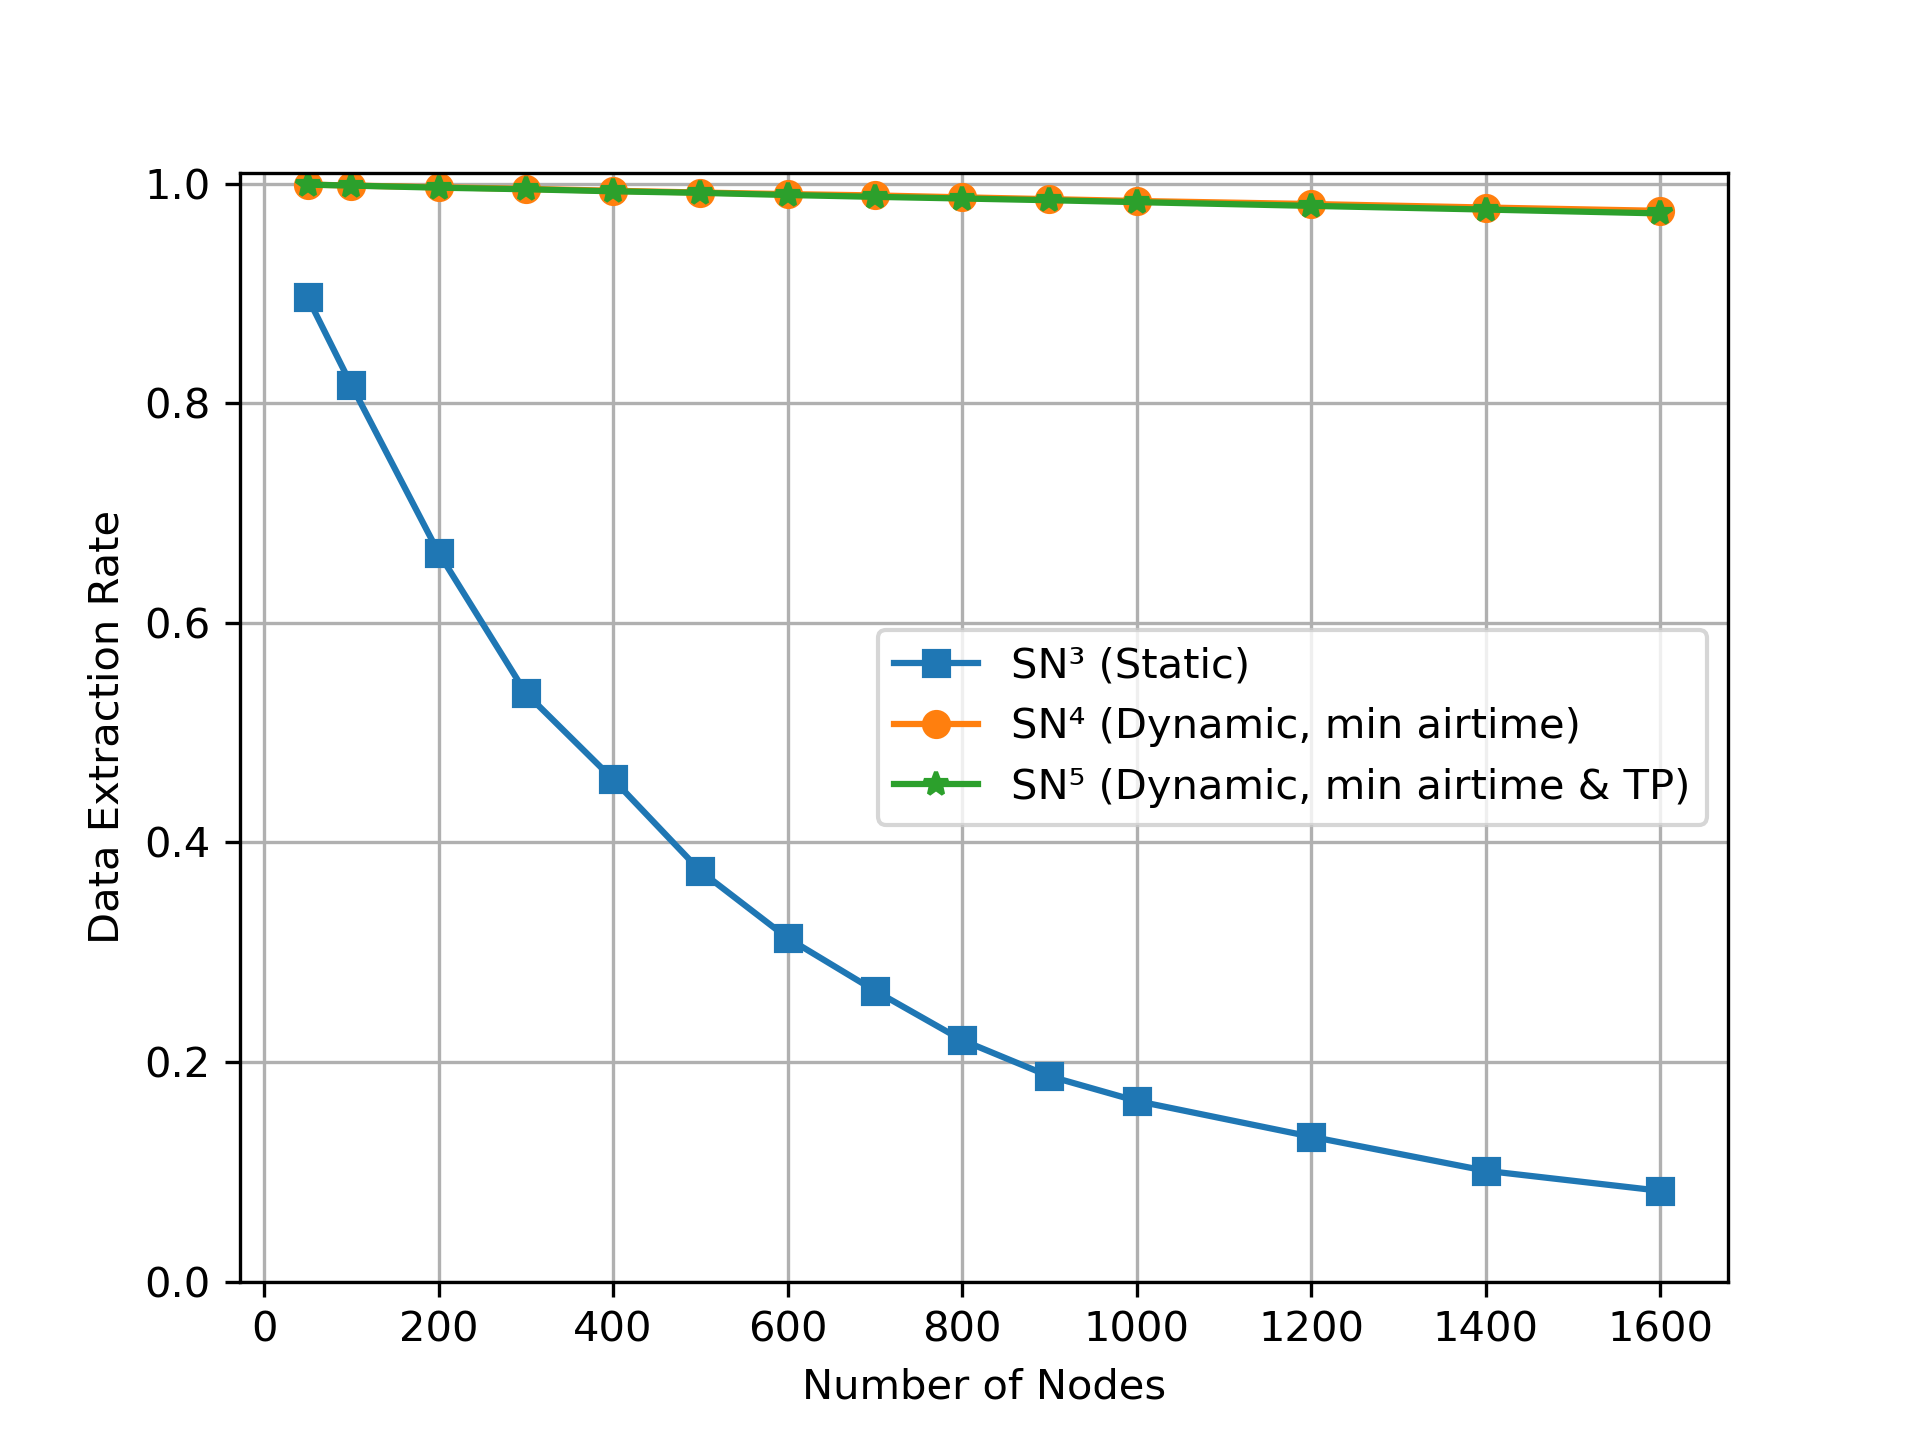
\includegraphics[width=10cm]{../res/python-f5-updated}
\end{center}

\smallskip

Also, being the \textbf{outdoor yard much larger than the underground one}, a long-range technology has the additional benefit of requiring a single technical and communicative deployment, rather than replicating it with a shorter range one, that could, however, provide additional benefits and simplicity to the underground area, as mentioned.

\smallskip

An ideal fit for such a layout is therefore represented by \textsc{LoRaWAN} or \textsc{LoRa-based} custom point-to-point technologies.

\subsection{The Things Network and The Things Stack}\label{ttn}

\textsc{The Things Network} (TTN) is an open-source infrastructure (and network server, the most intelligent part of a LoRa network) aiming at providing free LoRaWAN network coverage.

\smallskip

The project is actively maintained by a growing community across the world, on a voluntary basis.

\smallskip

Gateways are incrementally being deployed across the globe, providing an increasing network coverage.

\medskip

\textsc{The Things Network} plays, more or less, the same role that a mobile radio network operator plays for mobile User Terminals: it provides the user with the connectivity and managerial services of their LoRaWAN provisions.

\medskip

An implicit assumption of the underground environment, however, is that network coverage cannot be directly provided by \textsc{The Things Network}'s gateways: we will probably have to install a new one ourselves, also exploiting mains power being freely available.

\medskip

The gateway will also need network connectivity to forward collected measurements to either a local or remote data broker (e.g. MQTT).

\begin{itemize}
    \item If cable connectivity (e.g. \textsc{Ethernet}) is a viable option, we could directly exploit it and forward collected data to a remote processing broker, similarly to the inspected \textsc{ThingSpeak} implementation.
    \item If instead, only mains power is directly available, we could also add a \textsc{LoRaWAN Network Server}.

        Thankfully, the organization behind \textsc{The Things Network} open sourced its \textsc{Network Server} implementation (\href{https://github.com/TheThingsNetwork/lorawan-stack}{\texttt{"The Things Stack"}}), making it freely available to all interested entities for both global and small networks.
\end{itemize}

\smallskip

Furthermore, the hardware costs for \textsc{LoRa gateways and Network Servers} are decreasing more and more, becoming a quite affordable solution for modern implementations.

\smallskip

Finally, the installation should take care of physical and communicative protection of the device and, if necessary, inspect transmission characteristics with one or multiple sink nodes.

\subsection{Localization strategy}\label{localization-strategy}

Depending on the required precision and liveness metrics of the overall system, both \textsc{Triangulation} and \textsc{Fingerprinting} localization strategies can be applied to our case.

\medskip

In the \textsc{Triangulation} case, an additional number of anchor nodes is required in the environment: they are, in practice, inactive nodes, that just serves the purpose of providing the target with a distance estimation to perform triangulation with an adequate rate.

\smallskip

If mains power can also be provided to the anchor nodes, they should constitute the ideal solution.

\smallskip

In case mains power is not available, a maintenance strategy should be adopted in this case and the \textsc{fingerprinting} approach would benefit from the easier implementation strategy: note, however, that the overall precision will always be affected by the accuracy of the initial \textsc{fingerprinting database} construction.

\medskip

Our assumption, in the following, is that mains power is also available for anchor nodes to perform triangulation locally to the micro-controller node: in such a case, transmission parameters can also be adapted accordingly.

\smallskip

Measurement rate is assumed to live in the order of tens of seconds: much greater than the \textsc{LoRaWAN} optimized case.

\smallskip

The average speed of a forklift is assumed to reach, at its maximum, $\sim 10\ km/h$: an aggressive transmission rate should not be useful, in such a case.

\smallskip

Ultimately, optimizations on the effective machine's movement and directionality should be further taken into consideration, as shown in the \hyperref[pseudocode]{final pseudocode snippet}.

\smallskip

A small \textsc{versioning system} should therefore be simulated by the data management procedures.

\subsection{Data-exchange approach}\label{data-exchange}

As shown during the \textsc{Challenge} activities, both \textsc{MQTT} and \textsc{HTTP} or \textsc{CoAP} protocols are adequate for our case: they are all normally employed in the IoT field and, since our expected payload size would not represent a problem for either of those, all three can be quite equally chosen.

\smallskip

An ideal fit should therefore mimic the scenario inspected when using \textsc{ThingSpeak}, whose aim, among data collection, also resides in powerful data processing through \textsc{MATLAB} technologies.

\smallskip

Our assumption, in the following, is therefore to use the \textsc{MQTT} or \textsc{MQTT-SN} protocols, that also put an additional strength towards the IoT scenario, also optimizing on message sizes and transport management.

\section{Backend data processing and storage solution}

A forklift node exchanges planning is provided in the following, correlated by an ideal data management pipeline.

\begin{itemize}
    \item RSSI: integrated in all LoRaWAN messages, it is used to perform triangulation through the \hyperref[triangulation]{model-based localization approach described}.
    \item Directionality, speed and orientation: collected by the Inertial Measurement Unit (IMU), they are used also to implement a sketched versioning system, detecting meaningful changes for updates.
    \item Distance from obstacles: collected by the Ultrasonic distance sensor, they are used to implement the impact detection strategy, which also serves the purpose of providing the maintenance teams with useful insights about potential impacts.
    \item Additional tracking and status support information: collected, for example, by the GPS communication module if GPS coverage is found to be sufficient (e.g. in the outdoor yard).

        Interesting additional pieces of information are represented, for example, by a periodic battery status update, to plan for docking stations usage.
\end{itemize}

Ultimately, upon docking/charging procedures, an internal storage flush can be performed, to complete monitoring outcomes and solve eventually unavailable measurements due to communicative inabilities (collisions, congestion, \dots).

\medskip

Depending on \textsc{LoRa} coverage and cabling availability, both the \textsc{Gateway} and \textsc{Network Server} can be deployed remotely, exploiting, for example, \textsc{The Things Network}'s provisioning, \hyperref[ttn]{as mentioned}.

\smallskip

Our assumption, in the following, is that connectivity to \textsc{The Things Network}'s Network Server is available through appropriate cabling, while the \textsc{LoRa Gateway} should be deployed locally, due to poor coverage of the underground area.

\medskip

The \textsc{MQTT} data broker can be deployed both locally or remotely, depending, most likely, on the bandwith availability and storage requirements of the overall solution.

\smallskip

Our assumption, in the following, is that the \textsc{MQTT data broker} is deployed remotely, through a cloud service provider, that can also provide for additional reliability and scalability of the overall solution.

\medskip

The cloud service provider will therefore also manage data storage and maintenance, presumably replicating collected measurements both locally to the datacenter, through \textsc{RAID} storage solutions and consequently distributing it in a geographically-meaningful fault tolerance strategy.

\section{Overall system architecture}

The resulting overall system's architecture sketch is provided in the following, alongside the planned delivery paths and the assumed implementation details.

\begin{center}
    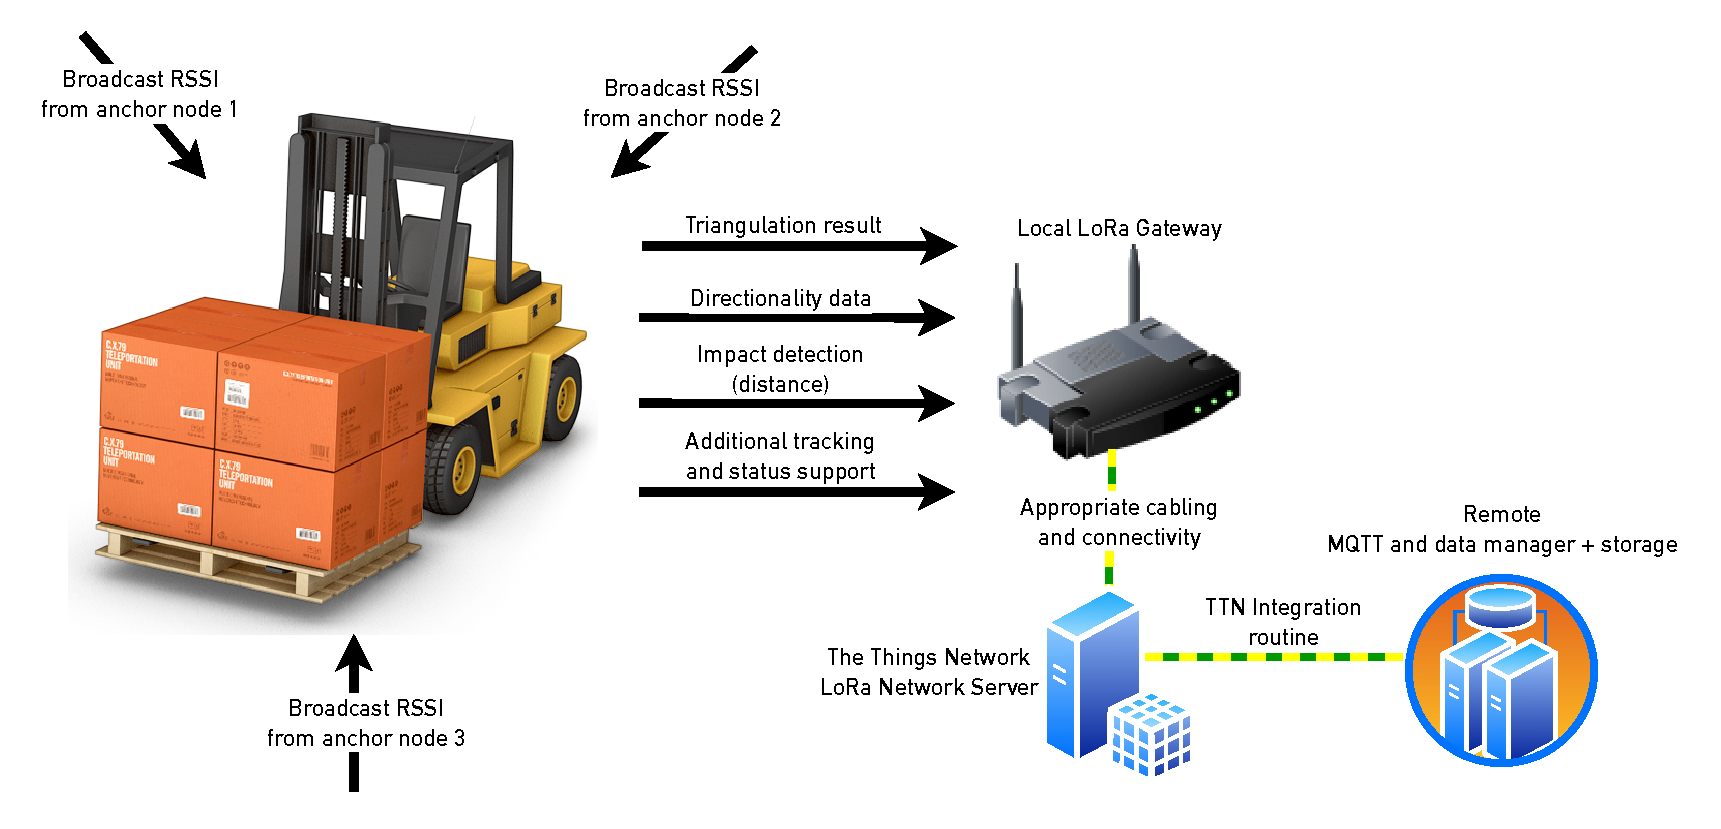
\includegraphics[width=18cm]{../res/communication-forklift}
\end{center}

The described solution ultimately empathizes on:

\begin{itemize}
    \item Simplicity: no more than a micro-controller/development board per forklift should be expected.

        A single LoRa gateway is expected to cover the whole underground area. Depending on the physical characteristics and coverage of the warehouse, additional ones could be required for the outdoor yard, if \textsc{The Things Network}'s coverage is not expected.

        Processing details are covered by \textsc{The Things Network}'s integration and a supporting cloud provider, which resolves the need for additional processing and data storage management.

        It finally ensures a reasonable accuracy for both the localization and monitoring requirements, through the strategically positioned anchor nodes.
    \item Low cost: \textsc{LoRa} end-nodes (micro-controller/development boards) and \textsc{Gateways} are becoming more and more affordable, though they may require an additive term due to the proprietary modulation scheme.
    \item Scalability: \hyperref[challenge-lorasim]{As also inspected} during the latest \textsc{Challenge} activity, \textsc{LoRaWAN} deployments can hugely benefit from optimizations on airtime through configuration of transmit parameters, as shown by the experimental run through \textsc{LoRaSim}, that exhibits a \textsc{Data Extraction Rate (DER)} $\geq 0,9$ in highly polluted transmission environments, while also covering considerable distances ($\sim$ hundreds meters).

        The outdoor yard, \hyperref[communication]{as mentioned}, may require additional \textsc{LoRa Gateways}, to both ensure additional stability and localization accuracy, via triangulation.
\end{itemize}

\section{Forklift logic: pseudocode snippet}\label{pseudocode}

\begin{minted}{C}
#include <IMU.h>  // Inertial Measurement Unit (IMU) library
#include <LoRaWAN.h>

LoRaModem modem;

void setup() {
    Serial.begin(115200);

    modem.begin(EU868);
    modem.joinOTAA(appEui, appKey);

    // additional transmission parameters...
    // in case of a custom gateway implementation, transmission intervals can be
    // lowered...
    Serial.println("Setup completed!");
}

bool computeImpact() {
    digitalWrite(PIN_TRIGGER, LOW);
    delayMicroseconds(2);
    digitalWrite(PIN_TRIGGER, HIGH);
    delayMicroseconds(10);
    digitalWrite(PIN_TRIGGER, LOW);

    // Read the pulse duration and compute the proportion:
    int duration = pulseIn(PIN_ECHO, HIGH);

    float distance = duration / 58.0;  // floating point division

    return (distance > DISTANCE_DISCRIMINANT);
}

const ANCHOR_NODES = 3;  // number of anchor nodes (>= 3, see theory)
float triangulation_RSSI[ANCHOR_NODES];
float previous_position[2];  // (x, y)
float current_position[2];

float IMU_accelerometer_measurements[3];
float IMU_gyroscope_measurements[3];
const PREVIOUS_OUTCOMES_VERSIONS = 5;  // versioning system implementation
float previous_IMU_outcomes[PREVIOUS_OUTCOMES_VERSIONS];
float current_IMU_outcome;

Forklift forklift;
int assigned_docking_station;

void loop() {
    enum GPS_coverage = check_GPS_coverage();
    if (GPS_coverage == GOOD) {
        current_position = get_GPS_position();
    } else {
        // Perform triangulation
        for (int i = 0; i < ANCHOR_NODES; i++) {
            // collect the RSSI from broadcast anchor nodes' transmissions
            triangulation_RSSI[i] = collect_RSSI(i);
        }

        // And finally compute an output position (x, y)
        current_position = triangulate(triangulation_RSSI);
    }

    // Let's now use the Inertial Measurement Unit to collect directionality
    IMU_accelerometer_measurements[0] = IMU.getAccelerometerOffset(X_AXIS);
    IMU_accelerometer_measurements[1] = IMU.getAccelerometerOffset(Y_AXIS);
    IMU_accelerometer_measurements[2] = IMU.getAccelerometerOffset(Z_AXIS);
    IMU_gyroscope_measurements[0] = IMU.getGyroOffset(X_AXIS);
    IMU_gyroscope_measurements[1] = IMU.getGyroOffset(Y_AXIS);
    IMU_gyroscope_measurements[2] = IMU.getGyroOffset(Z_AXIS);

    // And finally compute a meaningful outcome from the IMU
    current_IMU_outcome = compute_IMU_model(IMU_accelerometer_measurements,
                                            IMU_gyroscope_measurements);
    // In which we assumed a meaningful mathematical model describing the IMU's
    // measurements have been collectively used to come out with a final outcome

    // Let's implement a sketched versioning system: we will first compute the
    // average of the previous 5 measurements coming out of the IMU
    float previous_IMU_avg = 0;
    for (int i = 0; i < PREVIOUS_OUTCOMES_VERSIONS; i++) {
        previous_IMU_avg += previous_IMU_outcomes[i];
    }
    previous_IMU_avg /= PREVIOUS_OUTCOMES_VERSIONS;

    // and check for meaningful differences coming out of the IMU, impact
    // detection, triangulation or GPS tracking
    bool meaningful_difference_IMU =
        compare_IMU(previous_IMU_avg, current_IMU_outcome);
    bool meaningful_difference_position =
        euclidean_distance(current_position, previous_position);
    bool impact_detected = computeImpact();
    bool battery_status = forklift.battery.getStatus();

    if (meaningful_difference_IMU || meaningful_difference_position ||
        impact_detected) {
        msg = {
            IMU_outcome = current_IMU_outcome,
            position = current_position,
            impact = impact_detected,
            battery = battery_status
        }

        modem.beginPacket();
        modem.print(msg);
        modem.endPacket(true);
    }

    // And finally update local storage for the next versioning cycle
    update_local_state(current_IMU_outcome, current_position, impact_detected, battery_status);

    // return back to the docking station if battery status is poor
    if (battery_status == LOW) {
        forklift.move(assigned_docking_station);
    }

    delay(...);
}
\end{minted}

\end{document}